\documentclass[czech,a4paper,12pt]{article}[]

\usepackage{myDocument}
\usetikzlibrary{positioning, automata, calc}
\tikzstyle{accepting}=[path picture={%
  \draw let 
    \p1 = (path picture bounding box.east),
    \p2 = (path picture bounding box.center)
    in
      (\p2) circle (\x1 - \x2 - 2pt);
  }]
\lstset{xleftmargin=.3\textwidth, xrightmargin=.3\textwidth}
\renewcommand{\lstlistingname}{Kód}

\begin{document}

\begin{center}
\LARGE{Vysoké učení technické v Brně \\
Fakulta informačních technologií}
\vfill 
\LARGE{Dokumentace projektu z předmětu IFJ a IAL}\\
\Huge{\textbf{Implementace překladače jazyka IFJ20}}\\
\vfill
\large{\textbf{Tým 101, varianta I}\\
\begin{tabular}{ r l c}
\textbf{Jakšík, Aleš} & \textbf{(\texttt{xjaksi01})} & \textbf{25\%} \\ 
Vlasáková, Nela & (\texttt{xvlasa14}) & 25\% \\  
Mráz, Filip & (\texttt{xmraz01}) & 25\% \\
Bělohlávek, Jan & (\texttt{xbeloh08}) & 25\% 
\end{tabular}
}\\[3em]
5. 12. 2020
\end{center}

\newpage

\tableofcontents

\newpage

\section{Úvod}
Zadáním projektu bylo vytvořit překladač imperativního jazyka IFJ20 a na jeho vytvoření se podíleli všichni členové týmu. Naživo jsme se viděli jen jednou, pravidelně jsme však komunikovali pomocí Messengeru a hovory jsme realizovali na společném Discordovém serveru. Práci jsme si rozdělili následovně:

\paragraph{Aleš Jakšík}
\begin{inpar}
Vedoucí týmu dostal na práci syntaktickou a sémantickou analýzu vyjma analýzu výrazů, navíc také implementoval tabulku symbolů.

\medskip
\textbf{Soubory:}
    \begin{itemize}
    \item \texttt{parser.c/parser.h}
    \item \texttt{symtable.c/symtable.h}
\end{itemize}
\end{inpar}

\paragraph{Nela Vlasáková}
\begin{inpar}
Na práci dostala syntaktickou a sémantickou analýzu výrazů, k čemuž patří i implementace obousměrně vázaného seznamu.dokumentaci a testování kódu.

\medskip
\textbf{Soubory:}
\begin{itemize}
    \item \texttt{expression.c/expression.h}
    \item \texttt{exprList.c/exprList.h}
\end{itemize}
\end{inpar}    

\paragraph{Filip Mráz}
\begin{inpar}
Na starost dostal generování výsledného kódu a implementaci dynamického řetězce, dále se podílel na implementaci obousměrně vázaného seznamu pro lexikální analyzátor.

\medskip
\textbf{Soubory:}
\begin{itemize}
    \item \texttt{generator.c/generator.h}
    \item \texttt{tokenList.c/tokenList.h}
    \item \texttt{dynamicString.c/dynamicString.h}
\end{itemize}
\end{inpar}

\paragraph{Jan Bělohlávek}
\begin{inpar}
Honzovým úkolem bylo vytvořit lexikální analyzátor, pro který také vytvořil konečný automat.

\medskip
\textbf{Soubory:}
\begin{itemize}
    \item \texttt{scanner.c/scanner.h}
\end{itemize}
\end{inpar}

\newpage
\section{Návrh}
Celý překladač je složen z několika spolupracujících modulů. Každý má většinou jednu hlavní funkci, která je z jiného modulu volána, a tak tedy dojde k jakési komunikaci a předání informací. Kromě vrácení návratové hodnoty mohou takové funkce také zapisovat do různých proměnných (pomocí předání ukazatele na danou proměnnou), a oznamovat tak jiným modulům různé skutečnosti, příkladem by mohlo být například získání datového typu výrazu. Chybová návratová hodnota je předávána vždy zpět od místa, kde se vyskytla, až do \texttt{main.c}, kde je vyhodnocena, je na standartní chybový výstup vytištěna chybová hláška a program je ukončen s touto předávanou hodnotou.

\smallskip
K implementaci jsme využili dvou datových struktur - \textbf{binárního stromu} (pro tabulku symbolů) a \textbf{oboustranně vázaného seznamu}, který je používán jak pro nahrání celého vstupního souboru, tak například pro předávání výrazů k analýze, nebo následně předání výrazu ve formě postfixu k tištění. 

\smallskip
Pro lexikální analýzu jsme využili \textbf{konečného automatu}, při syntaktické kontrole jsme využili LL-gramatiky a \textbf{metody rekurzivního sestupu}. Výrazy jsme zpracovali podle \textbf{precedenční syntaktické analýzy}.


\section{Implementace}
Jako první je ze souboru \texttt{main.c} volán syntaktický/sémantický analyzátor - \texttt{parser.c}. Ten si zavolá lexikální analyzátor (jde tedy o syntaxí řízený překlad), který projde celý vstupní soubor, provede lexikální analýzu podle konečného automatu a vytvoří obousměrně vázaný seznam S tzv. \emph{Tokeny}. 

\begin{figure}[h!]
    \begin{lstlisting}[language=C, caption={Implementace struktury tokenu}, captionpos=b]
typedef struct Token {
    TokenType t_type;
    tStr *atribute;
    struct Token *lptr;
    struct Token *rptr;
} *TokenPtr;
    \end{lstlisting}
\label{tokenCode}
\end{figure}

Tento seznam pak předá zpět syntaktickému/sémantickému analyzátoru, který jej projde a provede syntaktickou kontrolu podle LL gramatiky, následně pak zkontroluje sémantiku. Pokud narazí na místo, kde by se měl nacházet výraz, vytvoří z něj další obousměrně vázaný seznam a pošle jej na precedenční analýzu do \texttt{expression.c}, kde je výraz zkontrolován jak po sémantické, tak syntaktické stránce, a v případě, že je vše v pořádku, je vstupní seznam reprezentující výraz převeden na postfix a odeslán dále do generátoru výstupního kódu.

\newpage


\subsection{Lexikální analýza - \texttt{scanner.c}}
Lexikální analýza je řízena konečným automatem. Ze vstupu načte vždy jeden znak a postupně je přidává do předem připraveného řetězce, dokud nedojde do stavu, kdy může tento řetězec přijmout nebo zamítnout. Pokud jej může přijmout, vytvoří z něj \emph{Token} a přidá jej do obousměrně vázaného seznamu, který poté, co narazí na \texttt{EOF}, považuje soubor za lexikálně korektní a předá jej zpět do \texttt{parser.c}.

\begin{center}
    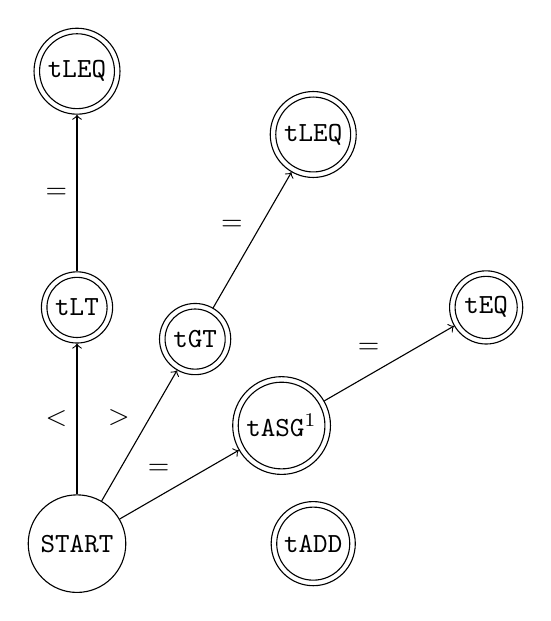
\begin{tikzpicture}[double distance=2pt,auto] 
        % START
        \node[state] (start)   {\texttt{START}}; 

        % LT -> LEQ branch
        \node[state, accepting] (lt) at (90:3) {\texttt{tLT}};   % LT
        \node[state, accepting] (leq) at (90:6) {\texttt{tLEQ}};  % LEQ

        % GT -> GEQ branch
        \node[state, accepting] (gt) at (60:3) {\texttt{tGT}};     % GT
        \node[state, accepting] (geq) at (60:6) {\texttt{tLEQ}};    % GEQ

        % ASSIGN -> EQ branch
        \node[state, accepting] (assign) at (30:3) {\texttt{tASG\footnotemark}};     % ASSIGN
        \node[state, accepting] (eq) at (30:6) {\texttt{tEQ}};    % EQ
        
        % +, -, *
        \node[state, accepting] (plus) at (0:3) {\texttt{tADD}};
        \path[->] 

        (start) edge node {$<$} (lt)
        (lt) edge node {$=$} (leq)
        (start) edge node {$>$} (gt)
        (gt) edge node {$=$} (geq)
        (start) edge node {$=$} (assign)
        (assign) edge node {$=$} (eq);
    \end{tikzpicture}
\end{center}
\footnotetext[1]{zkráceno z \texttt{tASSIGN} kvůli velikosti}

\subsubsection{Dynamický řetězec}
Práci s řetězci máme řešenou pomocí implementace vlastního dynamického řetězce.

\newpage

\subsection{Syntaktická a sémantická analýza}
Syntaktická kontrola je řízena pravidly \textbf{LL gramatiky}, informace potřebné k sémantické kontrole (existence proměnných a funkcí, datové typy a podobně) jsou uchovávány v \textbf{tabulce symbolů} implementované pomocí binárního stromu. 


\subsubsection{Syntaktická analýza}
Začátkem syntaktické analýzy je kontrola, jestli vstupní soubor obsahuje povinnou hlavičku. Následně se celý seznam, který obsahuje \emph{Tokeny} reprezentující vstupní soubor, projde poprvé. Funkce \texttt{buidInFunc} projde všechny hlavičky funkcí, uloží je do tabulky symbolů spolu s informacemi o vstupních a výstupních parametrech (počet a datový typ). Také zkontroluje, že poslední funkcí je \texttt{main}. Po provedení tohoto prvního běhu se pak celý seznam projde znova a kontrolují se těla jednotlivých funkcí. Tato kontrola se řídí pravidly LL gramatiky.

\subsubsection{Sémantická analýza}
Při procházení těly funkcí se do tabulky symbolů nahrávají informace o proměnných. Každé tělo představuje novou tabulku symbolů a postup vytváření tabulek je následující:

\begin{enumerate}
    \item \textbf{Vstup do těla} (funkce, konstrukce \texttt{if}, cyklus)
    \item \textbf{Vytvoří se nová tabulka symbolů} a vloží se do seznamu tabulek symbolů (vždy na první místo)
    \begin{itemize}
        \item Hlavička cyklu je vždy samostatná nová tabulka, tudíž je zaručeno, že v ní lze použít proměnné definované dříve a zároveň, že proměnné definované v hlavičce budou dostupné v jejím těle
    \end{itemize}
    \item \textbf{Odchod z těla} znamená odstranění tabulky ze seznamu tabulek symbolů
\end{enumerate}

Ověření, že nějaká proměnná již byla definována (a případné získání datového typu a podobně), pak vypadá tak, že se první podíváme do tabulky na začátku seznamu, a pokud nic nenajdeme, jdeme hlouběji, dokud ji nenajdeme, v opačném případě pak nastává chyba.

\subsubsection{Precedenční analýza výrazů}
Hlavní funkcí analyzátoru výrazů je funkce \texttt{parseExp}. Ta obdrží seznam \emph{Tokenů}, podle kterého následně vytvoří vlastní seznam, kde jsou prvky identifikovány podle symbolů precedenční tabulce.

\begin{figure}[h!]
    \begin{lstlisting}[language=C, caption={Položka seznamu pro precedenční analýzu}, captionpos=b]
typedef struct ListItem {
    bool isZero;
    PtType ptType;
    DataType dType;
    struct ListItem *next;
    struct ListItem *prev;
} *item;
    \end{lstlisting}
\label{exprCode}
\end{figure}

\newpage

Celá precedenční analýza je řízena precedenční tabulkou. Ta je v kódu implementována jako dvourozměrné pole znaků:

\begin{center}
\catcode`\-=12
\begin{tabular}{| c | p{2.3em} | p{2.3em} | p{2.3em} | p{2.3em} | p{2.3em} | p{2.3em} | p{2.3em} | p{2.3em} | p{2.3em} |}
\hline
    & \multicolumn{9}{ c |}{\texttt{input}} \\\hline
    \multirow{9}{*}{\rotatebox[origin=c]{90}{\texttt{opStack}}} & &\centering\textbf{+} & \centering\textbf{-} & \centering\textbf{*} & \centering\textbf{/} & \centering\textbf{(} & \centering\textbf{)} & \centering\textbf{cmp} & \textbf{\;\;\,\$} \\\cline{2-10}
    & \centering\textbf{+} & \centering R & \centering R & \centering S & \centering S & \centering R & \centering S & \centering R & \;\;\,R\\\cline{2-10}
    & \centering\textbf{-} & \centering R & \centering R & \centering S & \centering S & \centering R & \centering S & \centering R & \;\;\,R\\\cline{2-10}
    & \centering\textbf{*} & \centering R & \centering R & \centering R & \centering R & \centering R & \centering S & \centering R & \;\;\,R\\\cline{2-10}   
    & \centering\textbf{/} & \centering R & \centering R & \centering R & \centering R & \centering R & \centering S & \centering R & \;\;\,R\\\cline{2-10}      
    & \centering\textbf{(} & \centering S & \centering S & \centering S & \centering S & \centering R & \centering S & \centering R & \;\;\,R\\\cline{2-10}   
    & \centering\textbf{)} & \centering S & \centering S & \centering S & \centering S & \centering S & \centering S & \centering S & \;\;\,E\\\cline{2-10}   
    & \centering\textbf{cmp} & \centering R & \centering R & \centering R & \centering R & \centering R & \centering E & \centering R & \;\;\,R\\\cline{2-10}   
    & \centering\textbf{\$} & \centering S & \centering S & \centering S & \centering S & \centering S & \centering S & \centering E & \;\;\,A\\\hline 
\end{tabular}            
\end{center}

Analýza pracuje se třemi seznamy:

\begin{enumerate}
    \item \texttt{input} reprezentující vstupní výraz
    \item \texttt{idStack}, do kterého se vkládají výrazů
    \item \texttt{opStack}, kam jsou vkládány operátory
\end{enumerate} 

\medskip
Proměnná, ať už jde o nějaký identifikátor, číslo, desetinný literál nebo řetězec, je klasifikováno jako \texttt{E} (tedy jako výraz). Pokud při procházení seznamem narazíme na prvek označný jako \texttt{E}, rovnou jej vložíme do příslušného seznamu. Samotný proces precedenční analýzy pak probíhá následovně:

\begin{enumerate}
\item Symbol z precedenční tabulky získáme vždy zadáním "souřadnic":
\begin{quote}
\texttt{precTable[x][y]}
\end{quote}
kde \texttt{x} reprezentuje symbol na konci seznamu \texttt{OpStack} a \texttt{y} reprezentuje symbol, na který se právě díváme ve vstupním seznamu.
\item Pokud dostaneme \texttt{R}, provedeme redukci
\item Pokud dostaneme \texttt{S}, provedeme přesunutí symbolu ze vstupu \texttt{input} na \texttt{opStack}
\item Pokud dostaneme \texttt{A}, kontrolujeme, konečné podmínky přijetí výrazu a pokud projdou v pořádku, výraz převádíme na postfix
\end{enumerate}

\medskip
Redukce je prováděna na základě následujících pravidel:

\begin{center}
\ttfamily{ 
\begin{tabular}{r r l c l l l }
&  & (E) & $\rightarrow$ & E & &\\
E + E & $\rightarrow$ & E &  & E - E & $\rightarrow$ & E \\
E / E & $\rightarrow$ & E & & E * E & $\rightarrow$ & E \\
E < E & $\rightarrow$ & E & & E > E & $\rightarrow$ & E \\
E >= E & $\rightarrow$ & E & & E <= E & $\rightarrow$ & E \\
E == E & $\rightarrow$ & E & & E != E & $\rightarrow$ & E \\
\end{tabular}}
\end{center}



\subsection{Generování kódů}
\end{document}